% ============================================================
% manuscript.tex
% Ghost Skill and Dynamic Fidelity in Multi-Horizon PM10 Forecasting
% P4 Evidence: Single rolling-origin series
% Evidence status: B_HIGH_SOURCE_PROVENANCE_PENDING
%
% Frozen experimental source commit: 95c9cbdc8c582f5657523c404afa58e61f5e1137
% Publication packaging commit:      f233a20ae7eb7411e84eaaa326c3aff87601f628
%
% DO NOT SUBMIT without completing all TODO AUTHOR items.
% ============================================================

\documentclass[12pt]{article}

% ----- Encoding and fonts -----
\usepackage[T1]{fontenc}
\usepackage[utf8]{inputenc}
\usepackage{lmodern}

% ----- Layout -----
\usepackage[margin=1in, a4paper]{geometry}
\usepackage{setspace}
\usepackage{graphicx}
\onehalfspacing

% ----- Tables -----
\usepackage{booktabs}
\usepackage{array}
\usepackage{tabularx}
\usepackage{multirow}
\usepackage{siunitx}
\sisetup{detect-weight=true, detect-family=true}

% ----- Math -----
\usepackage{amsmath}
\usepackage{amssymb}

% ----- Graphics -----
\usepackage{graphicx}

% ----- Links -----
\usepackage{hyperref}
\hypersetup{
  colorlinks=true,
  linkcolor=blue,
  citecolor=blue,
  urlcolor=blue
}

% ----- Natbib for author-year citations -----
\usepackage{natbib}
\bibliographystyle{plainnat}

% ----- Keywords macro -----
\providecommand{\keywords}[1]{\par\bigskip\noindent\textbf{Keywords:} #1}

% ============================================================
% TITLE AND AUTHORS
% ============================================================

\title{Ghost Skill in Multi-Horizon PM$_{10}$ Forecasting:\\
Positive Error-Based Skill with Collapsed Dynamic Fidelity\\
and Failed Event Representation}

\author{%
  Federico Garc\'ia Crespi\thanks{%
    Corresponding author.
    Department of Computer Engineering,
    Universidad Miguel Hern\'andez de Elche, Spain.
    \texttt{fedeg@umh.es}}
  \and
  Julio Alberto Ramos Mart\'inez\\
  Department of Statistics, Mathematics and Computer Science,\\
  Universidad Miguel Hern\'andez de Elche, Spain.
  \texttt{j.ramos@umh.es}%
}

\date{August 2026}

\begin{document}
\maketitle

% ============================================================
\begin{abstract}
Verification of deterministic PM$_{10}$ forecasts routinely relies on
persistence-relative root-mean-square error (RMSE) skill, yet a model
can achieve positive skill while its predicted trajectory has collapsed
to a near-constant signal, retaining neither day-to-day variability nor
exceedance events.

We evaluate two contrasting models---a gradient-boosted tree (LightGBM)
and a classical seasonal autoregressive model (SARIMA)---across four
forecast horizons ($h = 1, 6, 24, 48$~h) under a rolling-origin
evaluation protocol applied to a single hourly PM$_{10}$ series.
Continuous error skill, dynamic-fidelity metrics (variance retention,
temporal variability, amplitude ratio), and exceedance event metrics
(POD, CSI) are assessed jointly.

At $h = 48$~h, SARIMA achieves a pooled RMSE skill of $+0.1325$ relative
to persistence, yet retains only $0.37\%$ of observed variance (variance
retention $= 0.0037$), temporal variability collapses to $2.2\%$ of the
observed signal, and the model fails to detect any train-defined
exceedance event ($\mathrm{POD} = 0.000$, $\mathrm{CSI} = 0.000$).
This pattern---positive baseline-relative error skill coexisting with
severe loss of dynamic fidelity and failed event representation---defines
the \emph{ghost skill} diagnostic and replicates across 3 of 5 expanding
evaluation folds. Dynamic collapse and complete event failure occur in
all 5 of 5 folds. LightGBM, which lacks positive error skill at 48~h
($\mathrm{Skill}_\mathrm{RMSE} = -0.0793$), nevertheless detects
exceedances with $\mathrm{CSI} = 0.2144$ ($\mathrm{POD} = 0.3226$),
reversing the model-preference ranking between error-based and event-based
criteria.

These results illustrate that improvement in baseline-relative RMSE
does not, by itself, establish preserved dynamic or event fidelity.
The evidence is bounded to the evaluated single series and does not
support universal claims about SARIMA or about PM$_{10}$ forecasting
in general.
\end{abstract}

\keywords{forecast verification; PM$_{10}$ forecasting; ghost skill;
variance retention; dynamic fidelity; rolling-origin evaluation;
exceedance events; persistence baseline; model-preference reversal}

% ============================================================
\section{Introduction}
\label{sec:introduction}
% ============================================================

Daily and sub-daily PM$_{10}$ forecasts inform short-horizon
air-quality management, public-health communication, and episode
alert systems \citep{who2021,wilks2011}. In operational settings,
the practical value of a forecast depends on more than average error:
decisions triggered by exceedance thresholds require that forecasts
also reproduce meaningful concentration swings and identify likely
pollution events.

Persistence-relative RMSE skill is the standard summary for this
verification task \citep{hyndman2006}. Positive skill indicates that
a model reduces RMSE relative to the persistence baseline; it is a
necessary condition for operational improvement over the simplest
extrapolation. Point-forecast accuracy under squared-error loss summarizes pointwise
discrepancy but does not directly characterize the trajectory
variability of predictions \citep{gneiting2011,jolliffe2012}. Under
squared-error loss, the conditional mean is the optimal point forecast
\citep{gneiting2011}. This distinction motivates examining whether
improvements in pointwise error are accompanied by preservation of
trajectory variability and event representation at increasing forecast
horizons.

We refer to this evaluative decoupling as \emph{ghost skill}: a diagnostic
label for the empirical situation where positive baseline-relative error
skill coexists with marked loss of dynamic fidelity and event representation,
altering which forecast is preferred. Ghost skill is employed here strictly
as a diagnostic label for this observed pattern, not as a general property
of a model family or a universal forecasting law.

This paper characterises this diagnostic pattern empirically in a
rolling-origin evaluation of LightGBM and SARIMA forecasters over
a single hourly PM$_{10}$ series, at four forecast horizons
($h = 1, 6, 24, 48$~h). We evaluate three complementary dimensions:
(i) continuous error skill relative to causal persistence; (ii) dynamic
fidelity across variance, temporal variability, and amplitude metrics;
and (iii) exceedance event representation at a train-derived threshold.
The joint reading of these dimensions identifies a model-preference
reversal at the 48-h horizon and supports the ghost-skill diagnosis for
48-h SARIMA in this evaluated series.

The contribution of this paper is narrowly evaluative: it does not
introduce new models, new datasets, or new training objectives. It
demonstrates that complementary evaluation dimensions---dynamic fidelity
and event representation---can yield a different model assessment from
error-based skill alone, in the evaluated single-series setting.

% ============================================================
\section{Data and Evaluation Setting}
\label{sec:methods}
% ============================================================

\subsection{Series and Preprocessing}
\label{sec:data}

The study evaluates an hourly PM$_{10}$ series preserved in the audited
forecasting archive. Because complete station-level metadata are not
embedded in the canonical row-level prediction schema, the empirical
evidence is evaluated and reported strictly as a single-series benchmark.

The evaluation uses a lags-only autoregressive setting without
meteorological covariates, applying causal feature processing within
the training window of each fold. A common-support filter restricts
comparative evaluations to identical matched forecast--observation
timestamps across models for each horizon, avoiding horizon composition
artefacts.

\subsection{Rolling-Origin Evaluation Protocol}
\label{sec:rolling_origin}

Forecasts are evaluated under a rolling-origin (time-series
cross-validation) protocol with five expanding folds
\citep{tashman2000,bergmeir2018}. In each fold, the training window
expands chronologically; a fixed test window immediately follows each
training window. No future information enters any training window:
all preprocessing steps, including threshold computation, are fitted
exclusively on the training partition of each fold and applied to
the corresponding test partition \citep{kaufman2012}.

Fold-wise metrics are computed independently for each fold and then
pooled across folds to produce the primary reported values. Pooled and
fold-wise statistics are kept strictly separate throughout and are
never conflated.

\subsection{Models}
\label{sec:models}

Two models are evaluated:

\begin{itemize}
\item \textbf{LightGBM}: A gradient-boosted decision tree model
  with lag features as predictors, trained under direct multi-step
  strategy (one model per horizon). No meteorological covariates
  are used.
\item \textbf{SARIMA}: A seasonal autoregressive integrated
  moving-average model specified as a sparse classical baseline.
  It is included as a statistical comparator to test whether the
  skill--fidelity tension is specific to machine learning or also
  appears in classical time-series modelling.
\end{itemize}

Both models are assessed at horizons $h \in \{1, 6, 24, 48\}$~h.
The persistence baseline predicts the last observed value at each
horizon.

\subsection{Metrics}
\label{sec:metrics}

\paragraph{Error-based skill.}
The persistence-relative RMSE skill at horizon $h$ is
\begin{equation}
  \label{eq:skill_rmse}
  \mathrm{Skill}_\mathrm{RMSE}(h)
    = 1 - \frac{\mathrm{RMSE}_\mathrm{model}(h)}{\mathrm{RMSE}_\mathrm{persistence}(h)},
\end{equation}
where both RMSEs are computed over matched forecast--observation pairs
within the common-support window. Positive values indicate that the
model reduces RMSE relative to persistence.

\paragraph{Dynamic fidelity.}
Four non-redundant dynamic-fidelity indicators are evaluated at
each horizon:
\begin{enumerate}
  \item \textbf{Variance retention}:
    $\alpha(h) = \operatorname{Var}(\hat{y}_h) / \operatorname{Var}(y_h)$,
    the ratio of predicted to observed variance over matched pairs.
    Both variances use population variance ($\mathrm{ddof}=0$).
  \item \textbf{Temporal variability}:
    $\tau(h) = \overline{|\Delta\hat{y}_h|} \,/\, \overline{|\Delta y_h|}$,
    the ratio of mean absolute one-step differences computed
    intra-fold between contiguous observations.
  \item \textbf{Amplitude ratio}:
    $\beta(h) = \mathrm{IQR}_{95\text{--}5}(\hat{y}_h) / \mathrm{IQR}_{95\text{--}5}(y_h)$,
    the ratio of the 90th-percentile interquantile ranges.
  \item \textbf{Event amplitude retention}:
    $\gamma(h) = \overline{\hat{y}_h[y_h > p_{75}]} \,/\,
    \overline{y_h[y_h > p_{75}]}$,
    the ratio of mean predicted to mean observed concentration
    over observation-defined exceedance events.
\end{enumerate}
Note that $\alpha(h)$, the standard-deviation ratio
$\sigma_{\hat{y}} / \sigma_{y}$ (reported as \texttt{std\_ratio}),
and the KGE variability component $\alpha_\mathrm{KGE}$ are
algebraically related expressions of dispersion attenuation;
they are not independent lines of evidence and are not treated
as such.

\paragraph{Exceedance event representation.}
Exceedance events are defined by the training-partition 75th
percentile threshold ($p_{75}$), estimated independently in each fold
using only training-window observations. Event representation is
evaluated by:
\begin{itemize}
  \item \textbf{POD} (Probability of Detection):
    $\mathrm{TP} / (\mathrm{TP} + \mathrm{FN})$.
  \item \textbf{CSI} (Critical Success Index):
    $\mathrm{TP} / (\mathrm{TP} + \mathrm{FP} + \mathrm{FN})$.
  \item \textbf{Event bias}:
    $(\mathrm{TP} + \mathrm{FP}) / (\mathrm{TP} + \mathrm{FN})$.
\end{itemize}

\paragraph{Ghost-skill diagnostic.}
Ghost skill is present diagnostically when: (1) baseline-relative
error skill is positive; (2) predictions show material degradation
across non-redundant dimensions of dynamic fidelity; and (3) the
degradation changes the scientific or operational conclusion.
Rank reversal between evaluation criteria is a manifestation of
this pattern, not the definition itself. The full diagnostic pattern
requires conditions (1)--(3) to hold jointly.

\subsection{Multi-Fold Stability Criterion}
\label{sec:fold_stability}

The fold-stability assessment reports how many of the five expanding
folds satisfy each diagnostic condition individually.
Pooled variance retention and fold-wise variance retention (median,
minimum, maximum) are reported separately and are never conflated.
The ghost-skill diagnostic pattern is evaluated fold-by-fold; its
replication count across folds (3 of 5 at $h = 48$~h) quantifies
the structural stability of the finding within this series.

% ============================================================
\section{Results}
\label{sec:results}
% ============================================================

\subsection{Error-Based Forecast Skill}
\label{sec:results_error_skill}

Evaluating models strictly by RMSE relative to the causal persistence
baseline reveals strong horizon dependence in forecast skill
(Table~\ref{tab:error_metrics}).

At $h = 1$~h, LightGBM ($\mathrm{RMSE} = 5.6668$~$\mu$g\,m$^{-3}$)
yields slightly negative skill ($\mathrm{Skill}_\mathrm{RMSE} = -0.0104$)
relative to persistence ($\mathrm{RMSE} = 5.6086$~$\mu$g\,m$^{-3}$),
whereas SARIMA ($\mathrm{RMSE} = 5.4328$~$\mu$g\,m$^{-3}$) achieves
a small positive skill ($\mathrm{Skill}_\mathrm{RMSE} = +0.0314$).
At $h = 6$~h, LightGBM reaches its maximum relative error skill
($\mathrm{Skill}_\mathrm{RMSE} = +0.0729$,
$\mathrm{RMSE} = 9.1465$~$\mu$g\,m$^{-3}$) against a persistence
RMSE of $9.8654$~$\mu$g\,m$^{-3}$; SARIMA achieves
$\mathrm{Skill}_\mathrm{RMSE} = +0.0827$
($\mathrm{RMSE} = 9.0499$~$\mu$g\,m$^{-3}$).

At extended horizons, the two models diverge. LightGBM continuous
error skill falls below persistence at $h = 24$~h
($\mathrm{Skill}_\mathrm{RMSE} = -0.0343$,
$\mathrm{RMSE} = 12.8018$~$\mu$g\,m$^{-3}$) and remains negative at
$h = 48$~h ($\mathrm{Skill}_\mathrm{RMSE} = -0.0793$,
$\mathrm{RMSE} = 15.2283$~$\mu$g\,m$^{-3}$). SARIMA maintains positive
skill across both extended horizons, attaining
$\mathrm{Skill}_\mathrm{RMSE} = +0.0450$ at $h = 24$~h
($\mathrm{RMSE} = 11.8194$~$\mu$g\,m$^{-3}$ vs persistence
$12.3770$~$\mu$g\,m$^{-3}$) and $\mathrm{Skill}_\mathrm{RMSE} = +0.1325$
at $h = 48$~h ($\mathrm{RMSE} = 12.2409$~$\mu$g\,m$^{-3}$ vs
persistence $14.1099$~$\mu$g\,m$^{-3}$). Evaluated exclusively by
continuous root-mean-square error, SARIMA appears superior at extended
lead times.

\begin{table}[ht]
\centering
\caption{Continuous error metrics by model and horizon.
$\mathrm{Skill}_\mathrm{RMSE} = 1 - \mathrm{RMSE}_\mathrm{model} /
\mathrm{RMSE}_\mathrm{persistence}$; positive values indicate
improvement over causal persistence.
Source: \texttt{pub\_table\_1\_error\_metrics.csv}, experimental commit
\texttt{95c9cbd}.}
\label{tab:error_metrics}
\begin{tabular}{llSSS}
\toprule
Model & Horizon (h) &
  {RMSE ($\mu$g\,m$^{-3}$)} &
  {Persistence RMSE ($\mu$g\,m$^{-3}$)} &
  {$\mathrm{Skill}_\mathrm{RMSE}$} \\
\midrule
LightGBM & 1  & 5.667 & 5.609 & -0.0104 \\
LightGBM & 6  & 9.147 & 9.865 & +0.0729 \\
LightGBM & 24 & 12.802 & 12.377 & -0.0343 \\
LightGBM & 48 & 15.228 & 14.110 & -0.0793 \\
\addlinespace
SARIMA   & 1  & 5.433 & 5.609 & +0.0314 \\
SARIMA   & 6  & 9.050 & 9.865 & +0.0827 \\
SARIMA   & 24 & 11.819 & 12.377 & +0.0450 \\
SARIMA   & 48 & 12.241 & 14.110 & +0.1325 \\
\bottomrule
\end{tabular}
\end{table}

\subsection{Dynamic Fidelity and Variance Collapse}
\label{sec:results_dynamic_fidelity}

Dynamic fidelity metrics reveal that positive continuous error skill
can coexist with severe structural attenuation of predicted
time-series variability (Table~\ref{tab:dynamic_fidelity}).

LightGBM retains substantial dynamic variability at $h = 48$~h
(variance retention $= 0.8659$, temporal variability $= 0.3856$),
despite its negative error skill at that horizon. SARIMA, by contrast,
undergoes progressive attenuation across horizons. At $h = 24$~h, SARIMA
retains $2.86\%$ of observed variance (variance retention $= 0.0286$),
with temporal variability dropping to $0.1530$ and amplitude ratio
to $0.1734$.

At $h = 48$~h, SARIMA undergoes near-total dynamic collapse: pooled
variance retention falls to $\mathbf{0.0037}$ ($\mathbf{0.37\%}$),
temporal variability to $\mathbf{0.0223}$ ($2.2\%$), and amplitude
ratio to $\mathbf{0.0626}$ ($6.3\%$). Rather than capturing
high-frequency concentration dynamics, 48-h SARIMA predictions collapse
toward a near-constant trajectory despite outperforming persistence
in continuous RMSE. Variance retention ($0.0037$), standard-deviation
ratio (\texttt{std\_ratio} $= 0.0604$), and KGE variability
($\alpha_\mathrm{KGE} = 0.0604$) are algebraically related expressions
of the same dispersion attenuation and are not treated as independent
evidence.

\begin{table}[ht]
\centering
\caption{Dynamic-fidelity metrics by model and horizon.
Variance retention $= \operatorname{Var}(\hat{y}) / \operatorname{Var}(y)$;
temporal variability $= \overline{|\Delta\hat{y}|} / \overline{|\Delta y|}$;
amplitude ratio $= \mathrm{IQR}_{95\text{--}5}(\hat{y}) /
\mathrm{IQR}_{95\text{--}5}(y)$;
event amplitude retention $= \overline{\hat{y}[y>p_{75}]} /
\overline{y[y>p_{75}]}$.
Source: \texttt{pub\_table\_2\_dynamic\_fidelity.csv}, experimental commit
\texttt{95c9cbd}.}
\label{tab:dynamic_fidelity}
\begin{tabular}{llSSSS}
\toprule
Model & Horizon (h) &
  {Var.\ retention} &
  {Temp.\ variability} &
  {Amplitude ratio} &
  {Event amp.\ retention} \\
\midrule
LightGBM & 1  & 0.689 & 0.696 & 0.824 & 0.859 \\
LightGBM & 6  & 0.551 & 0.456 & 0.711 & 0.773 \\
LightGBM & 24 & 0.599 & 0.495 & 0.791 & 0.720 \\
LightGBM & 48 & 0.866 & 0.386 & 1.160 & 0.666 \\
\addlinespace
SARIMA   & 1  & 0.798 & 0.764 & 0.899 & 0.898 \\
SARIMA   & 6  & 0.357 & 0.503 & 0.598 & 0.714 \\
SARIMA   & 24 & 0.029 & 0.153 & 0.173 & 0.544 \\
SARIMA   & 48 & 0.004 & 0.022 & 0.063 & 0.507 \\
\bottomrule
\end{tabular}
\end{table}

\subsection{Exceedance Event Representation}
\label{sec:results_event_representation}

Forecast capability for PM$_{10}$ exceedances degrades rapidly
for models exhibiting dynamic variance collapse
(Table~\ref{tab:event_metrics}). Exceedance events are defined by
the training-partition 75th percentile threshold, computed
independently within each fold.

At $h = 6$~h, LightGBM retains active event detection capabilities
($\mathrm{POD} = 0.585$, $\mathrm{CSI} = 0.450$,
event bias $= 0.886$), while SARIMA retains moderate event
representation ($\mathrm{POD} = 0.534$, $\mathrm{CSI} = 0.425$,
event bias $= 0.791$). By $h = 24$~h, SARIMA event detection has
degraded substantially ($\mathrm{POD} = 0.099$, $\mathrm{CSI} = 0.095$,
event bias $= 0.138$).

At $h = 48$~h, SARIMA experiences complete event detection failure:
$\mathrm{TP} = 0$, $\mathrm{FP} = 0$, $\mathrm{FN} = 1153$,
$\mathrm{TN} = 2799$, yielding $\mathbf{\mathrm{POD} = 0.000}$ and
$\mathbf{\mathrm{CSI} = 0.000}$ (event bias $= 0.000$). Although
48-h SARIMA achieves positive continuous RMSE skill
($\mathrm{Skill}_\mathrm{RMSE} = +0.1325$), it issues no threshold
exceedance alerts across the entire evaluation sample.

\begin{table}[ht]
\centering
\caption{Exceedance event metrics by model and horizon.
Threshold: training-partition 75th percentile (computed per fold).
POD: Probability of Detection ($\mathrm{TP}/(\mathrm{TP}+\mathrm{FN})$);
CSI: Critical Success Index ($\mathrm{TP}/(\mathrm{TP}+\mathrm{FP}+\mathrm{FN})$);
Event bias: $(\mathrm{TP}+\mathrm{FP})/(\mathrm{TP}+\mathrm{FN})$.
Source: \texttt{pub\_table\_3\_event\_metrics.csv}, experimental commit
\texttt{95c9cbd}.}
\label{tab:event_metrics}
\begin{tabular}{llSSSSSS}
\toprule
Model & Horizon & TP & FP & FN & TN & {POD} & {CSI} \\
\midrule
LightGBM & 1  &  966 &  220 &  283 & 2712 & 0.773 & 0.658 \\
LightGBM & 6  &  727 &  374 &  515 & 2545 & 0.585 & 0.450 \\
LightGBM & 24 &  571 &  532 &  639 & 2329 & 0.472 & 0.328 \\
LightGBM & 48 &  372 &  582 &  781 & 2217 & 0.323 & 0.214 \\
\addlinespace
SARIMA   & 1  &  981 &  272 &  268 & 2660 & 0.785 & 0.645 \\
SARIMA   & 6  &  663 &  319 &  579 & 2600 & 0.534 & 0.425 \\
SARIMA   & 24 &  120 &   47 & 1090 & 2814 & 0.099 & 0.095 \\
SARIMA   & 48 &    0 &    0 & 1153 & 2799 & 0.000 & 0.000 \\
\bottomrule
\end{tabular}
\end{table}

\subsection{Model-Preference Reversal}
\label{sec:results_rank_reversal}

Discrepancies between continuous error skill and threshold-event
metrics lead to an explicit reversal in model preference at the 48-h
horizon (Table~\ref{tab:ghost_skill_structure} and Figure~\ref{fig:horizon_divergence}).

Ranking models by $\mathrm{Skill}_\mathrm{RMSE}$ at $h = 48$~h
favors SARIMA over LightGBM ($+0.1325$ vs $-0.0793$). Evaluating the
same aligned 48-h forecasts on event criteria reverses this model
ordering: LightGBM detects 372 of the 1,153 observed training-defined
$p_{75}$ events ($\mathrm{POD} = 0.3226$, $\mathrm{CSI} = 0.2144$),
whereas SARIMA detects none ($\mathrm{POD} = 0.0000$, $\mathrm{CSI} = 0.0000$).
Kendall's $\tau_b$ between the two 48-h prediction series was $0.236$,
providing an auxiliary measure of concordance between their temporal
rankings. In this evaluation, model selection governed solely by relative
RMSE prefers a forecast that captures none of the evaluated threshold
exceedances.

\begin{figure}[ht]
\centering
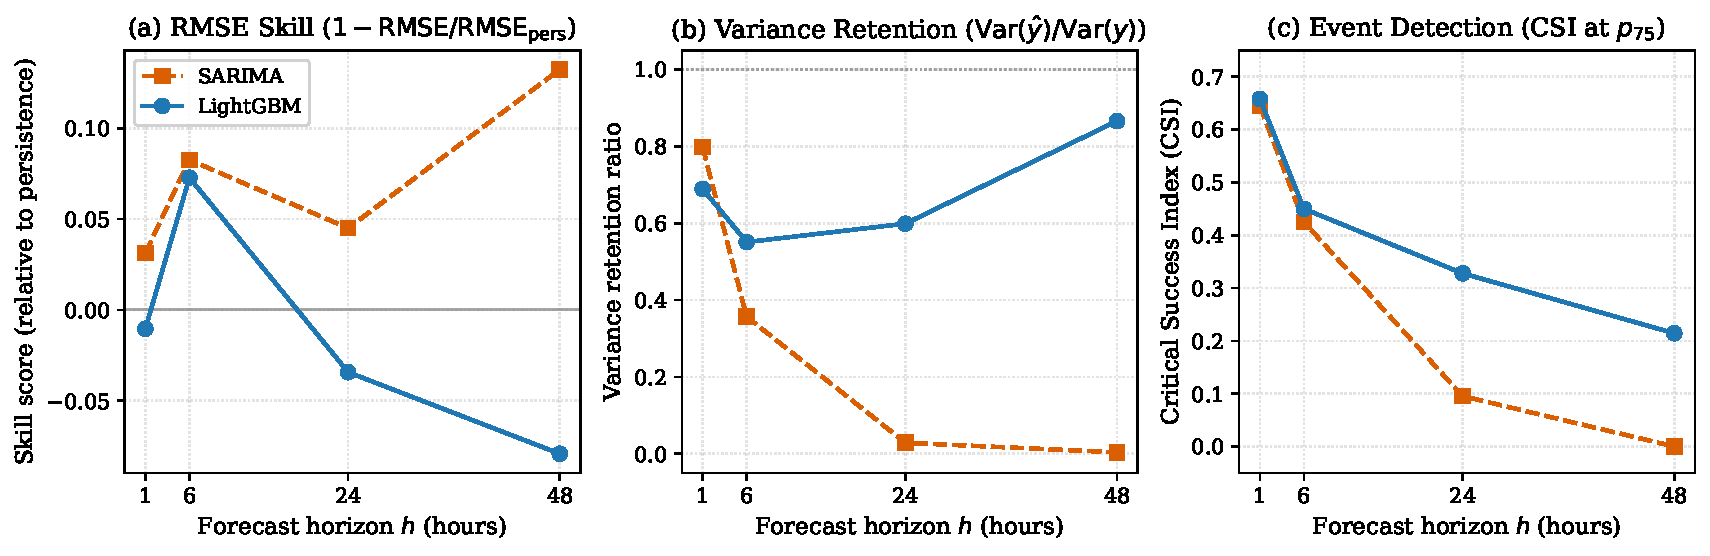
\includegraphics[width=\linewidth]{figures/fig1_horizon_evaluation_divergence.pdf}
\caption{Horizon-wise evaluation divergence between LightGBM and SARIMA across (a) persistence-relative RMSE skill, (b) variance retention, and (c) Critical Success Index (CSI) at the train-derived $p_{75}$ threshold. At $h=48$~h, RMSE skill favors SARIMA ($+0.1325$ vs $-0.0793$), while dynamic fidelity and threshold-event detection favor LightGBM ($\mathrm{CSI} = 0.2144$ vs $0.0000$). Source: \texttt{fig1\_horizon\_evaluation\_divergence.csv}, derived from publication source tables \texttt{pub\_table\_1\_error\_metrics.csv}, \texttt{pub\_table\_2\_dynamic\_fidelity.csv}, and \texttt{pub\_table\_3\_event\_metrics.csv}.}
\label{fig:horizon_divergence}
\end{figure}

\subsection{Multi-Fold Stability and Ghost-Skill Diagnosis}
\label{sec:results_fold_stability}

Multi-fold analysis confirms that dynamic collapse and complete event
failure in 48-h SARIMA forecasts are persistent features across the
five expanding evaluation folds (Table~\ref{tab:ghost_skill_structure}
and Figure~\ref{fig:fold_stability}).

Across all $5/5$ folds, 48-h SARIMA exhibits dynamic collapse
(\texttt{dynamic\_collapse\_all\_folds = True}; fold-wise variance
retention median $= 0.0007$ [$0.07\%$], range $[0.0005,\, 0.0012]$,
maximum fold value $= 0.12\%$) and complete event failure
(\texttt{complete\_event\_failure\_all\_folds = True};
$\mathrm{POD} = 0.0000$ and $\mathrm{CSI} = 0.0000$ in all 5 folds).
Positive continuous error skill ($\mathrm{Skill}_\mathrm{RMSE} > 0$)
is present in $3/5$ folds (median $= +0.1124$,
range $= [-0.3059,\, +0.2129]$).

The variance-collapse and event-failure components recur in all five
folds, whereas the complete three-criterion diagnostic pattern occurs
in three of five folds (\texttt{stability\_pattern = GHOST\_PATTERN\_REPLICATED\_3\_OF\_5\_FOLDS}).
In this rolling-origin evaluation, the 48-h SARIMA forecasts
satisfy the diagnostic definition of ghost skill
(\texttt{ghost\_skill\_status = GHOST\_SKILL\_DIAGNOSTIC\_SATISFIED\_IN\_RECOVERED\_SINGLE\_SERIES}).

\begin{figure}[ht]
\centering
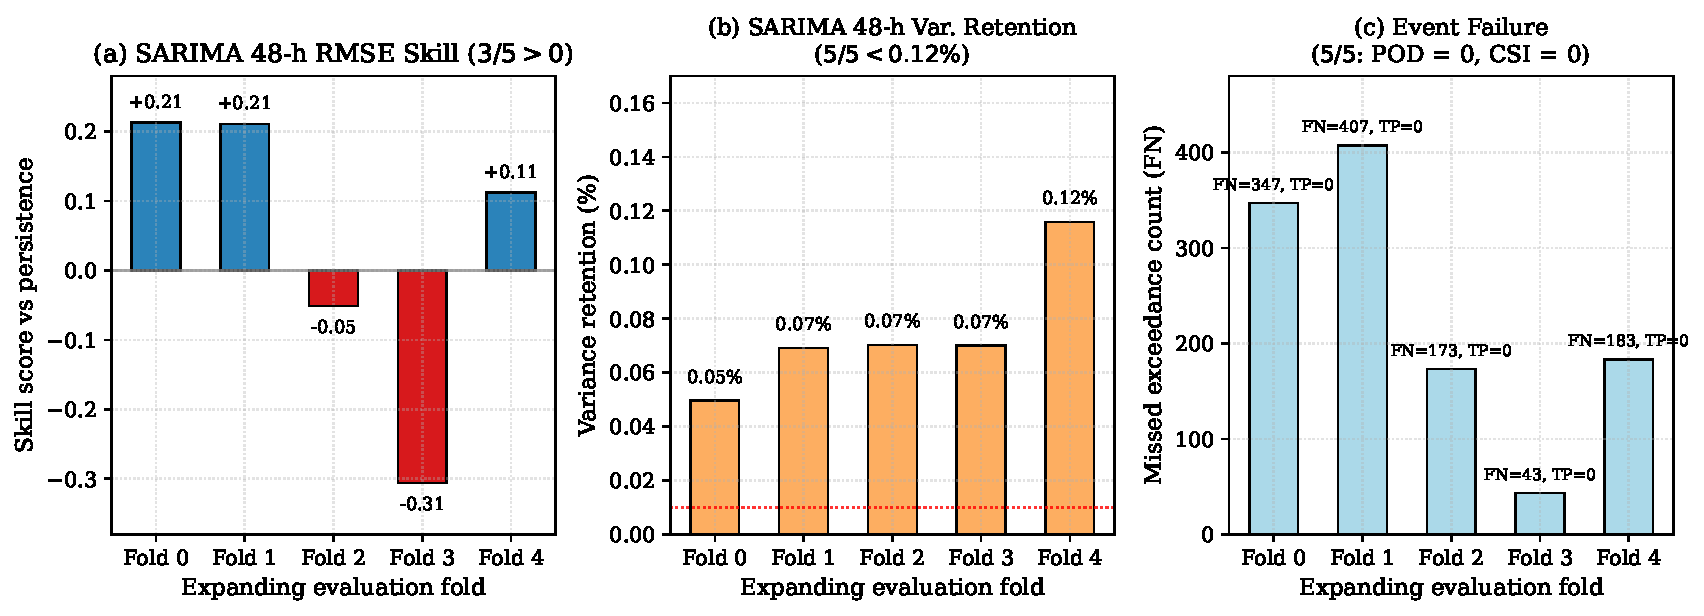
\includegraphics[width=\linewidth]{figures/fig2_sarima48_fold_stability.pdf}
\caption{Fold-wise evaluation of 48-h SARIMA forecasts across five expanding folds: (a) RMSE skill relative to persistence ($3/5 > 0$, median $+0.1124$), (b) variance retention ($5/5 \leq 0.12\%$, median $0.07\%$), and (c) missed exceedances at the train-derived $p_{75}$ threshold ($5/5$: $\mathrm{POD} = 0.0000$, $\mathrm{CSI} = 0.0000$, $\mathrm{TP} = 0$). The variance-collapse and event-failure components recur in all five folds, whereas the complete three-criterion diagnostic pattern occurs in three of five folds. Source: \texttt{fig2\_sarima48\_fold\_stability.csv}, derived from \texttt{fold\_stability\_by\_model\_horizon\_fold.csv}.}
\label{fig:fold_stability}
\end{figure}

\begin{table}[p]
\centering
\caption{Ghost-skill structure and fold-stability summary.
$\mathrm{Skill}_\mathrm{RMSE}$ and variance retention are pooled
over matching fold--horizon windows.
Fold-wise variance retention: median [min, max] across 5 folds,
reported only for $h \geq 24$~h where fold heterogeneity is material.
Source: \texttt{pub\_table\_4\_ghost\_skill\_structure.csv} and
\texttt{fold\_stability\_summary\_sarima.csv},
experimental commit \texttt{95c9cbd}.}
\label{tab:ghost_skill_structure}
\small
\begin{tabular}{%
  l
  l
  S[table-format=+1.4]
  S[table-format=1.4]
  S[table-format=1.4]
  S[table-format=1.4]
  l}
\toprule
Model & $h$ (h) &
  {$\mathrm{Skill}_\mathrm{RMSE}$} &
  {Var.\ ret.\ (pooled)} &
  {POD} &
  {CSI} &
  Ghost-skill status \\
\midrule
LightGBM & 1  & -0.0104 & 0.689 & 0.773 & 0.658 &
  Negative skill \\
LightGBM & 6  & +0.0729 & 0.551 & 0.585 & 0.450 &
  Moderate degradation; events retained \\
LightGBM & 24 & -0.0343 & 0.599 & 0.472 & 0.328 &
  Negative skill \\
LightGBM & 48 & -0.0793 & 0.866 & 0.323 & 0.214 &
  Negative skill \\
\addlinespace
SARIMA   & 1  & +0.0314 & 0.798 & 0.785 & 0.645 &
  No ghost skill \\
SARIMA   & 6  & +0.0827 & 0.357 & 0.534 & 0.425 &
  No ghost skill \\
SARIMA   & 24 & +0.0450 & 0.029 & 0.099 & 0.095 &
  Strong candidate; fold heterogeneity \\
SARIMA   & 48 & +0.1325 & 0.004 & 0.000 & 0.000 &
  \textbf{Ghost skill: 3/5 folds} \\
\bottomrule
\multicolumn{7}{p{\linewidth}}{%
  \emph{Note}: At $h = 48$~h, SARIMA fold-wise variance retention:
  median $0.0007$ [$0.07\%$], range $[0.0005,\, 0.0012]$.
  Dynamic collapse in 5/5 folds; complete event failure in 5/5 folds;
  positive error skill in 3/5 folds; full ghost-skill pattern in 3/5 folds.}\\
\end{tabular}
\end{table}

% ============================================================
\section{Discussion}
\label{sec:discussion}
% ============================================================

\subsection{Error Skill Does Not Imply Dynamic or Event Fidelity}
\label{sec:disc_main}

The primary finding of this evaluation is that positive baseline-relative
RMSE skill does not necessarily coincide with preserved dynamic fidelity
or event representation. In the evaluated series, 48-h SARIMA achieves
its highest RMSE skill relative to persistence ($+0.1325$), yet
simultaneously exhibits low variance retention ($0.0037$), low step-to-step
temporal variability ($0.0223$), and detects zero training-defined
exceedance events ($0/1,153$). The diagnostic label \emph{ghost skill}
describes this specific coexistence: error-based skill relative to
persistence is positive, while dynamic and event metrics indicate severe
loss of dynamic fidelity and event representation.

This empirical pattern is consistent with long-horizon forecast attenuation
where average squared error relative to persistence decreases alongside
a loss of high-frequency variability; however, the present diagnostic
design does not isolate the model-internal mechanism responsible for
this attenuation.

This divergence is not confined to a single evaluation window.
The variance-collapse and event-failure components recur in all five
folds, whereas the complete three-criterion diagnostic pattern occurs
in three of five folds. At 24~h, a similar---though less extreme---tendency
is visible (variance retention $= 0.029$, $\mathrm{POD} = 0.099$),
consistent with a progressive loss of dynamic fidelity across extended
lead times. These 24-h results are reported as secondary supporting
evidence and are not the central diagnostic case.

The LightGBM--SARIMA comparison demonstrates the evaluative consequence
of this divergence: SARIMA is preferred under continuous RMSE skill
($+0.1325$ vs $-0.0793$), but LightGBM is preferred under $p_{75}$
event representation ($\mathrm{CSI} = 0.2144$ vs $0.0000$), changing
the resulting model ordering.

\subsection{Interpretive Boundaries}
\label{sec:disc_boundaries}

Several interpretive limits apply to the present findings.

\emph{Single-series scope and metadata provenance.}
The evidence derives from a single hourly PM$_{10}$ series evaluated
under a rolling-origin protocol. No station-aggregated, network-wide,
or multi-series claim is supported by this evidence. Whether ghost skill
occurs in other series, at other monitoring stations, or in other
pollutant contexts is an open empirical question.

\emph{No causal claim.}
The study does not test any mechanism linking RMSE optimisation to
variance collapse. The coexistence of positive RMSE skill and collapsed
variance is an empirical observation under the evaluated protocol; it
is not attributed to a training-objective cause.

\emph{No universal model claim.}
The finding that SARIMA at 48~h exhibits ghost skill in this series
does not imply that SARIMA generally produces ghost skill, nor that
any other model family is immune to this pattern.

\emph{Evidence grade.}
The evidence is assessed at grade B (high source provenance, pending
verification). The station metadata required for full provenance
verification was not available from the source parquet file at the
time of this analysis.

\subsection{Implications for Forecast Evaluation Practice}
\label{sec:disc_implications}

The present results suggest that verification of deterministic
PM$_{10}$ forecasts---and potentially of point forecasts in related
environmental and atmospheric contexts---is more informative when
error-based skill is read alongside dynamic-fidelity and event-based
diagnostics. A forecast that reduces average squared error relative
to persistence may still yield a near-constant trajectory with poor
episode sensitivity, in which case the error-based assessment is
insufficient to characterise operational utility \citep{gneiting2011,jolliffe2012}.

Reporting variance retention and exceedance metrics alongside standard
skill scores would make this potential divergence visible without
requiring additional model training or external data. The cost of such
reporting is low; the interpretive benefit---particularly in alert
contexts---is material when the evaluated series exhibits skill--fidelity
decoupling of the magnitude observed here.

% ============================================================
\section{Limitations}
\label{sec:limitations}
% ============================================================

This study is intentionally bounded in scope.

The empirical evidence covers a single hourly PM$_{10}$ series; transfer
to other pollutants, temporal resolutions, spatial scales, or national
networks is not assessed. The evaluation is restricted to two models
(LightGBM and SARIMA) as diagnostic contrasts; it is not a leaderboard
or a comprehensive survey of model families. The lags-only design
deliberately excludes meteorological covariates to isolate the
autoregressive signal; models with richer feature sets may exhibit
different skill--fidelity profiles.

The exceedance threshold is defined by the training-partition 75th
percentile, estimated per fold. The threshold choice affects event
counts; this is a diagnostic convention, not a regulatory definition.
The study does not use the WHO 24-hour PM$_{10}$ guideline value or
any statutory threshold as an alert benchmark.

The rolling-origin protocol uses five expanding folds. Results could
vary with different fold counts, test-window sizes, or training-window
lengths. The fold-wise evidence reported here is bounded to the
reported protocol design.

The ghost-skill diagnostic is defined operationally for this study.
It is not proposed as a universal verification standard, and the
three-criterion definition (positive skill, dynamic degradation,
changed assessment) is an analytic choice rather than a derived
theoretical necessity.

% ============================================================
\section{Conclusion}
\label{sec:conclusion}
% ============================================================

Evaluating PM$_{10}$ forecasts by persistence-relative RMSE skill alone
can favor a model that achieves error reduction while failing to capture
threshold-defined exceedance events. In the evaluated series, 48-h SARIMA
forecasts achieve $\mathrm{Skill}_\mathrm{RMSE} = +0.1325$ over persistence,
yet retain $0.37\%$ of observed variance and detect none of the 1,153
observed training-defined $p_{75}$ events ($\mathrm{POD} = 0.0000$,
$\mathrm{CSI} = 0.0000$) across all five rolling-origin folds. Conversely,
LightGBM yields negative error skill at 48~h ($-0.0793$) but retains
dynamic variability and detects 372 exceedance events ($\mathrm{CSI} = 0.2144$),
resulting in a reversal of model preference between continuous error and
event criteria.

These results illustrate that positive error-based skill does not
guarantee preserved dynamic fidelity or event representation. In pollutant
forecasting settings where episodic behavior is relevant alongside average
error, reporting dynamic-fidelity and event metrics alongside RMSE skill
provides complementary information for distinguishing error improvement
from preserved trajectory and event fidelity.

The empirical evidence is strictly bounded to the evaluated single-series
rolling-origin design and does not support generalizations to other
monitoring series or model architectures.

% ============================================================
\section*{Data and Code Availability}
\label{sec:data_availability}
% ============================================================

The analysis code, evaluation scripts, and frozen publication source
tables that underpin all numerical results in this manuscript are
openly available at
\url{https://github.com/fedeg-umh-es/varret-pm10-paper}.
The frozen experimental state corresponds to repository commit
\texttt{95c9cbdc8c582f5657523c404afa58e61f5e1137}; publication
table packaging corresponds to commit
\texttt{f233a20ae7eb7411e84eaaa326c3aff87601f628}.
The canonical input prediction file
(\texttt{predictions\_rolling\_origin.parquet},
SHA-256: \texttt{e7073712ba1ab9f3de29621dfa9c96eec634b86ad7bf66ae37a9c098d15b58c4})
and all derived publication source tables are archived in the repository
and can be used to reproduce every number reported in this manuscript
\citep{sandve2013}.

% ============================================================
\section*{CRediT Author Contributions}
% ============================================================

Federico Garc\'ia Crespi: Conceptualisation, Data curation,
Formal analysis, Investigation, Methodology, Software, Validation,
Visualisation, Writing -- original draft, Writing -- review
\& editing.
Julio Alberto Ramos Mart\'inez: Conceptualisation, Supervision,
Writing -- review \& editing.

% ============================================================
\section*{Declaration of Competing Interests}
% ============================================================

The authors declare that they have no known competing financial
interests or personal relationships that could have appeared to
influence the work reported in this paper.

% ============================================================
\section*{Acknowledgements}
% ============================================================

The authors used a generative AI assistant for language editing and
for \LaTeX{} and reference formatting. All data processing, analysis,
results, and scientific conclusions are the authors' own and were
verified by the authors, who take full responsibility for the content
of this paper.

% TODO AUTHOR: Insert funding statement (grant number(s) and
% funding body) before submission.

% ============================================================
% BIBLIOGRAPHY
% ============================================================

\bibliography{references}

\end{document}
